\documentclass[tikz, border = 0pt]{standalone}
\usetikzlibrary{arrows.meta, backgrounds}
\definecolor{orange}{HTML}{E89A68}

\begin{document}
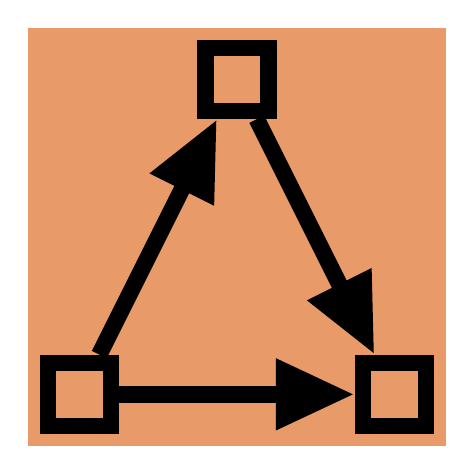
\begin{tikzpicture}

\tikzset{
background rectangle/.style = {fill = orange}, show background rectangle,
manifest/.style = {rectangle, line width = 6pt,  draw,  minimum width = 0.8cm, minimum height = 0.8cm},
regression/.style = {-{Triangle[length = 1cm]}, line width = 6pt},
	}
  
% Manifest
\node at (-2, -2) [manifest] (X) {};
\node at (2, -2) [manifest] (Y) {};
\node at (0, 2) [manifest] (M) {};

% Regressions
\path [regression] (X) edge [] (Y);
\path [regression] (X) edge [] (M);
\path [regression] (M) edge [] (Y);

\end{tikzpicture}
\end{document}